\section{Materiales y métodos}

\subsection{Datos}

\vspace{0,3cm}

\subsubsection*{Datos del fenotipo}

Para este estudio, se utilizó el fenotipo Demencia frontotemporal, identificado con el término HP:0002145 en Human Phenotype Ontology (HPO). A partir de este término HPO, se han extraído 52 genes asociados al fenotipo. Estos genes se obtuvieron mediante la API Ontology Annotation Network \cite{hpo_api} de HPO, que permite acceder programáticamente a las anotaciones entre términos fenotípicos y genes. A través de esta API, se descargaron los datos en formato JSON, que luego fueron procesados para extraer los nombres de los genes y guardarlos en un archivo TSV.

Estos genes, relacionados con el desarrollo de la demencia frontotemporal y otras patologías neurodegenerativas, representan el conjunto inicial de genes sobre el que se construirá la red de interacciones para el análisis posterior. Cada uno de ellos se identifica mediante su ID único en la base de datos de NCBIGene, lo cual facilita el acceso y la referencia a los datos genéticos específicos.

Para asegurar la reproducibilidad, se utilizó la versión 2.0.4 de HPO  \cite{HPO}, para obtener el término fenotípico y descargar los genes relacionados con el fenotipo de estudio. En la siguiente sección se proporciona una descripción detallada de HPO.
 
\subsubsection*{Human Phenotype Ontology (HPO)}

HPO proporciona una ontología estandarizada que describe anomalías fenotípicas observadas en enfermedades humanas, facilitando la identificación y análisis de genes asociados a diversas características clínicas. Cada término en HPO representa una anomalía específica, como la demencia frontotemporal, y está diseñado para facilitar la caracterización precisa de los fenotipos en el contexto de enfermedades hereditarias. La ontología se desarrolla y actualiza de forma continua utilizando fuentes como la literatura médica, así como bases de datos como Orphanet, DECIPHER y OMIM. Actualmente, HPO contiene más de 18,000 términos y ofrece más de 156,000 anotaciones asociadas a enfermedades hereditarias \cite{HPO}.


\subsubsection*{Datos de interacción}

Los datos de interacción representan conexiones funcionales y físicas entre proteínas, y constituyen la base para construir redes de interacción en el análisis de procesos biológicos. En este estudio, los datos de interacción proteína-proteína (PPI) fueron extraídos de la base de datos STRING mediante su API REST \cite{string_api}, que permite recuperar programáticamente redes de interacción específicas basadas en listas de genes o proteínas de interés.

A través de esta API, se obtuvieron las interacciones entre los genes asociados al fenotipo FTD (HP:0002145) en formato TSV. En este archivo, cada fila representa una interacción entre dos proteínas y contiene las siguientes columnas.

\begin{itemize}
	\item \textbf{protein1:} ID de la primera proteína en la interacción, precedido por el código taxonómico del organismo (por ejemplo, "9606" para proteínas humanas).
	\item \textbf{protein2:} ID de la segunda proteína en la interacción, también con el prefijo de organismo.
	\item \textbf{combined\_score:} Puntuación de confianza combinada para cada interacción proteína-proteína, con valores que oscilan entre 0 y 1000. Esta puntuación refleja la probabilidad de que una interacción sea real, basada en una integración de diversas fuentes de evidencia, como co-ocurrencia filogenética, co-expresión, minería de texto y datos experimentales. Cada tipo de evidencia se evalúa y puntúa individualmente, y luego se combina en el "combined\_score", proporcionando así un indicador global de confiabilidad para cada interacción funcional o física \cite{szklarczyk2023stringdb}.
\end{itemize}

Estos datos obtenidos se utilizarán para construir una red de interacciones entre los genes asociados al fenotipo FTD, permitiendo analizar las relaciones funcionales entre proteínas en este contexto. Esta red servirá como base para el análisis de clustering, facilitando la identificación de módulos de genes potencialmente implicados en funciones biológicas específicas.

Para asegurar la reproducibilidad del análisis, se utilizó la versión 12.0 de STRING, junto con su API REST de STRING para la extracción de interacciones.


\subsubsection*{STRING}
La base de datos STRING (Search Tool for the Retrieval of Interacting Genes/Proteins) es un recurso bioinformático diseñado para recopilar, organizar y analizar redes de interacciones proteína-proteína y asociaciones funcionales en cualquier genoma secuenciado. STRING integra información de diversas fuentes, como minería de texto científico, predicciones computacionales basadas en coexpresión y contexto genómico, y datos experimentales obtenidos de estudios de interacciones proteicas. Además, los usuarios pueden acceder a la base de datos para explorar redes de interacción, realizar análisis de enriquecimiento funcional y generar redes personalizadas para genomas específicos, facilitando así la investigación en biología celular y molecular. Actualmente, STRING cubre 59.309.604 proteínas provenientes de 12.535 organismos.  \cite{szklarczyk2023stringdb}.

\subsection{Software}

Para el análisis funcional y la construcción de redes genéticas en este estudio, se seleccionaron herramientas especializadas que permiten tanto la exploración bioinformática como la visualización de datos complejos. Dado que el objetivo principal es investigar la interacción entre genes y módulos específicos asociados a la demencia frontotemporal, se ha optado por una combinación de paquetes en Python y R que ofrecen un balance entre precisión analítica y capacidades visuales avanzadas.

\subsection*{Paquetes de Python para el análisis funcional y otras funciones}

\begin{itemize}
	\item \textbf{Pandas (versión 2.2.3)}: Este paquete proporciona estructuras de datos eficientes y flexibles, como DataFrames, que facilitan el procesamiento y manipulación de datos complejos. En el contexto de este estudio, Pandas permite organizar, filtrar y procesar resultados de enriquecimiento funcional, simplificando el manejo de grandes volúmenes de datos bioinformáticos \cite{pandas}.
	\item \textbf{Matplotlib (versión 3.8.1)}: Matplotlib es una librería de visualización muy versátil que soporta múltiples tipos de gráficos en 2D, lo que resulta útil para representar tendencias y relaciones entre genes en gráficos de líneas, barras, dispersión, y más. Este paquete se utilizará para visualizar los resultados de enriquecimiento y las interacciones génicas \cite{matplotlib}.
	\item \textbf{Scienceplots (versión 2.1.1)}: Este paquete extiende Matplotlib proporcionando estilos de gráficos estéticamente optimizados para publicaciones científicas. Con Scienceplots, se puede lograr una presentación visual de alta calidad, ideal para gráficos que requieren una apariencia profesional \cite{scienceplots}.
	\item \textbf{Requests (versión 2.31.0)}: Requests es una biblioteca para realizar solicitudes HTTP de manera simple y efectiva. En este estudio, se utiliza para conectar con APIs externas como la de STRINGdb, permitiendo la descarga automatizada de datos de redes y enriquecimiento \cite{requests}.
	\item \textbf{GOATOOLS (versión 1.2.3)}: Este paquete permite realizar análisis de enriquecimiento funcional en términos de Gene Ontology (GO), lo que facilita la identificación de términos GO sobre-representados en conjuntos de genes. Es una herramienta clave para comprender funciones biológicas asociadas a los genes estudiados \cite{goatools}.
	\item \textbf{G:Profiler (versión 1.4.0)}: G:Profiler realiza análisis de enriquecimiento funcional abarcando varias bases de datos (GO, KEGG, Reactome, entre otras). La versatilidad de este paquete lo convierte en una excelente opción para explorar las funciones biológicas de conjuntos de genes con una amplia cobertura de recursos \cite{gprofiler}.
	\item \textbf{Statsmodels (versión 0.14.0)}: Statsmodels es una biblioteca de estadística que permite aplicar ajustes de p-valor, como el método de Benjamini-Hochberg, para reducir el impacto de falsos positivos en los resultados de enriquecimiento. Esto asegura una interpretación estadísticamente robusta de los resultados \cite{statsmodels}.
\end{itemize}

\subsection*{Paquetes de R para clustering y visualización de redes}

\begin{itemize}
	\item \textbf{Cluster (versión 2.1.5)}: Este paquete ofrece una variedad de algoritmos clásicos de clustering (como k-means y clustering jerárquico), facilitando la agrupación de genes según patrones de expresión similares, lo cual es fundamental para identificar posibles módulos relacionados con la demencia frontotemporal \cite{cluster}.
	\item \textbf{Factoextra (versión 1.0.8)}: Factoextra permite una visualización clara y accesible de resultados de clustering, proporcionando gráficos intuitivos para explorar la estructura de los datos y resaltar posibles módulos o patrones de coexpresión \cite{factoextra}.
	\item \textbf{WGCNA (versión 1.71)}: Este paquete es ideal para detectar módulos de genes coexpresados mediante la construcción de redes de coexpresión genética ponderada, lo cual es útil en estudios de expresión génica complejos como el de la demencia frontotemporal \cite{wgcna}.
	\item \textbf{Igraph (versión 1.5.0)}: Igraph facilita la construcción, manipulación y visualización de redes genéticas y módulos de coexpresión. Este paquete es útil para analizar la conectividad y relación entre genes en un contexto de red \cite{igraph}.
	\item \textbf{STRINGdb (versión 2.10.0)}: STRINGdb es un paquete que conecta con la base de datos STRING, permitiendo realizar enriquecimiento funcional en redes y visualizar interacciones proteicas y genéticas. Es útil para identificar las relaciones funcionales entre genes \cite{stringdb}.
	\item \textbf{Pathview (versión 1.36.0)}: Este paquete permite integrar datos de expresión génica en rutas de KEGG, ofreciendo representaciones gráficas que muestran la implicación de los genes en rutas metabólicas y de señalización, lo cual es relevante para entender su rol en la enfermedad \cite{pathview}.
	\item \textbf{ClusterProfiler (versión 4.15.0)}: ClusterProfiler permite realizar análisis de enriquecimiento funcional de alta precisión en términos de GO, KEGG y Reactome. Ofrece opciones avanzadas de visualización y ajuste de p-valores, facilitando la interpretación de los resultados \cite{clusterprofiler}.
\end{itemize}

\subsection{Análisis de enriquecimiento de vías biológicas}

El análisis de enriquecimiento permite identificar vías biológicas o pathways que están significativamente representados en una lista de genes de interés, por medio de prubas estadísticas. Un pathway es un conjunto de genes que trabajan en conjunto para llevar a cabo un proceso biológico específico.\cite{Reimand2019}

Se realizó un análisis de enriquecimiento mediante la API de STRINGdb. Mediante el mapeo de las anotaciones funcionales de los genes en ontologías como Gene Ontology (GO), UniProt, Reactome y KEGG y comparando la distribución de estos términos en el conjunto de genes de interés con su distribución en un conjunto de referencia, se identificaron estadísticamente los términos sobrerrepresentados en la lista de genes asociados a la enfermedad. \cite{Tipney2010}

STRINGdb, por tanto, permite analizar diversas categorías de anotaciones funcionales, incluyendo los términos de Gene Ontology (procesos biológicos, funciones moleculares y componentes celulares), rutas de KEGG y Reactome \cite{szklarczyk2023stringdb}. Se realizó un filtrado según el tipo de término para obtener los diferentes enriquecimientos funcionales de interés.

Para calcular el enriquecimiento, STRINGdb utiliza un test hipergeométrico que evalúa si la representación de cada término funcional en el conjunto de genes de interés es mayor que la esperada por azar. Para controlar el error debido a comparaciones múltiples, se aplica la corrección de Benjamini-Hochberg para ajustar la tasa de descubrimiento falso (FDR) \cite{szklarczyk2023stringdb}.

El análisis de enriquecimiento se realizó tanto en el conjunto completo de genes asociados a la enfermedad, extraído de términos de HPO, como en los genes agrupados en clústeres. 


\subsection{Clustering}

Al aplicar algoritmos de clustering, nuestro objetivo es descubrir comunidades funcionales dentro de la red de genes asociada a la demencia frontotemporal. Estas comunidades, módulos, o \textit{clusters} funcionales pueden representar procesos biológicos específicos, vías celulares, o mecanismos asociados al fenotipo FTD. Encontrar estos clusters podría revelar posibles dianas terapéuticas o grupos de biomarcadores dentro del conjunto de genes, lo cual podría abrir las puertas a nuevos tratamientos para los pacientes de FTD.

\subsubsection*{Red}

En la red de interacción proteína-proteína (PPI) obtenida mediante la API de STRINGdb, cada nodo representa un gen y cada arista representa una interacción entre genes, ponderada por un puntaje de confianza otorgado por STRINGdb \cite{szklarczyk2023stringdb}. Para enfocarnos en interacciones más sólidas y confiables, se aplicó un umbral mínimo de confianza en las aristas, lo que permitió refinar la red y mejorar la relevancia de los clústeres detectados 

% (\textbf{NOTA:} Se debe ahondar en esto si al final se hace: ¿Por qué ese umbral? ¿Y si fueran otros umbrales?).

\subsubsection*{Algoritmos}

A continuación, se detallan los tres algoritmos de clustering, proporcionados por la librería \textit{iGraph}, elegidos para este estudio, los cuales pretenden cubrir diferentes enfoques teóricos en la detección de comunidades funcionales \cite{igraph}.  

\textit{Walktrap}: Algoritmo de clustering jerárquico aglomerativo que detecta comunidades basándose en la probabilidad de que recorridos aleatorios dentro de la red permanezcan dentro de clústeres cohesivos \cite{pons2005walktrap}. El algoritmo aplica recorridos aleatorios para capturar la proximidad de los nodos, asumiendo que los nodos que pertenecen a la misma comunidad tienen mayores probabilidades de estar conectados mediante recorridos cortos. Comienza con cada nodo como su propio clúster, fusionando sucesivamente los clústeres cercanos hasta alcanzar una partición óptima. Se ajustó la longitud de los pasos (\textit{steps}).

\textit{Algoritmo de Leiden}: Se basa en optimizar el Constant Potts Model (CPM) de la red \cite{traag2019leiden,constantplottsmodel}. Esta función, mostrada en la Ecuación \ref{eq:cpm}, evalúa la calidad de una partición en comunidades considerando un balance entre la densidad interna de cada clúster y el parámetro de resolución \(\gamma\), que controla el tamaño preferido de las comunidades finales. El término \(n_c\) se refiere al número de nodos, mientras que \(e_c\) es el número de aristas internas, ambos referidos a la comunidad \(c\).

\begin{equation}
	\label{eq:cpm}
	\mathcal{H} = \sum_{c} \left[ e_c - \gamma \left( \frac{n_c (n_c - 1)}{2} \right) \right]
\end{equation}

\noindent Se ajustó el parámetro \(\gamma\), así como el número de iteraciones del algoritmo, permitiendo que el Leiden refinara iterativamente la partición. El resto de parámetros se fijaron a su valor por defecto. 

% (\textbf{NOTA:} Hay un parámetro intersante, \textit{initial\_membership} el cual son nodos 'semilla' que se pasan como argumento, y el algoritmo intenta mejorar las comunidades alrededor de estos nodos. Podríamos usar genes del análisis funcional como semilla y ver qué pasa.)

\textit{Algoritmo de Louvain}: Este algoritmo optimiza la modularidad de la red, una métrica que mide la calidad de una partición en comunidades al comparar la densidad de conexiones internas con la densidad esperada si las conexiones fueran aleatorias \cite{Blondel2008Louvain}. La modularidad \( Q \), definida en la Ecuación \ref{eq:modularity}, es un valor escalar entre \(-1\) y \(1\) que representa la diferencia entre la densidad de aristas dentro de las comunidades y la densidad de aristas esperada. El algoritmo Louvain maximiza esta modularidad en dos fases, cuyo resultado es la formación una nueva red sobre la cual se repite el proceso hasta que la modularidad no mejore más. En redes ponderadas, los autores del algoritmo expresaron la modularidad a optimizar como:

\begin{equation}
	\label{eq:modularity}
	Q = \frac{1}{2m} \sum_{i,j} \left[ A_{ij} - \frac{k_i k_j}{2m} \right] \delta(c_i, c_j),
\end{equation}

\noindent donde \( A_{ij} \) es el peso de la arista entre los nodos \( i \) y \( j \), \( k_i \) y \( k_j \) son las sumas de los pesos de las aristas conectadas a los nodos \( i \) y \( j \), \( c_i \) y \( c_j \) representan las comunidades a las que pertenecen los nodos \( i \) y \( j \), y \( \delta(c_i, c_j) \) es una función delta de Kronecker que es 1 si \( c_i = c_j \) y 0 en caso contrario. El término \( m \) es la suma total de los pesos de las aristas en la red.

\noindent Se ajustó el parámetro de resolución, que controla el tamaño final de las comunidades. El resto de parámetros se dejaron con sus valores por defecto.

\subsubsection*{Medidas de Rendimiento}

Como se comentó anteriormente, el principal objetivo del clustering en nuestra red PPI es determinar las comunidades funcionales subyacentes con la finalidad de identificar rutas metabólicas compatibles con la elaboración de dianas o biomarcadores para el tratamiento de la FTD. Por esto, no se debe perder la interpretabilidad biológica de la red, a la vez que se intenta maximizar la calidad del clustering aplicado. Dadas estas condiciones, se propone una optimización multiobjetivo, repartiendo las tareas de significancia biológica y calidad del clustering entre las siguientes métricas:

\begin{itemize}
	\item \textit{Modularidad (Q)}. Destinada a la evaluación de la calidad del clustering aplicado. Valores altos indican una conectividad interna densa dentro de los clústeres y conexiones dispersas entre ellos. La alta modularidad sugiere comunidades bien definidas.
	
	\item \textit{Puntaje de Enriquecimiento Funcional}: Para cada clúster, se realizó un análisis de enriquecimiento funcional mediante STRINGdb. Este puntaje refleja la significancia estadística de pathways, términos de la Ontología de Genes u otras anotaciones funcionales enriquecidas dentro de los clústeres. Un puntaje alto indica mayor relevancia biológica, ya que los clústeres enriquecidos en términos específicos probablemente representan procesos biológicos significativos.
\end{itemize}


\subsubsection*{Optimización}
Se generaron varias configuraciones de modelos al ajustar sistemáticamente los parámetros de los algoritmos y evaluamos cada configuración en base a modularidad y puntaje de enriquecimiento funcional. Al trazar estos puntajes en un frente de Pareto, identificamos las configuraciones que representan el mejor equilibrio entre coherencia estructural (modularidad) y relevancia biológica (enriquecimiento funcional) \cite{goodarzi2014PARETOFRONT1,jahan2013multiPARETOFRONT2,costa2015paretoPARETOFRONT3}. Las configuraciones a lo largo de esta frontera representan soluciones Pareto-eficientes de clustering, donde mejorar una métrica no compromete significativamente la otra, permitiendo explorar soluciones con un balance diferente de las métricas de rendimiento elegidas.

% \textbf{NOTA:} Podríamos aplicar algún algoritmo interesante de ajuste de los hiperparámetros, yo (Mario) tengo experiencia aplicando Tree-structured Parzen Estimator y otros algoritmos de ajuste Bayesiano en Python.

\begin{figure}[h]
	\centering
	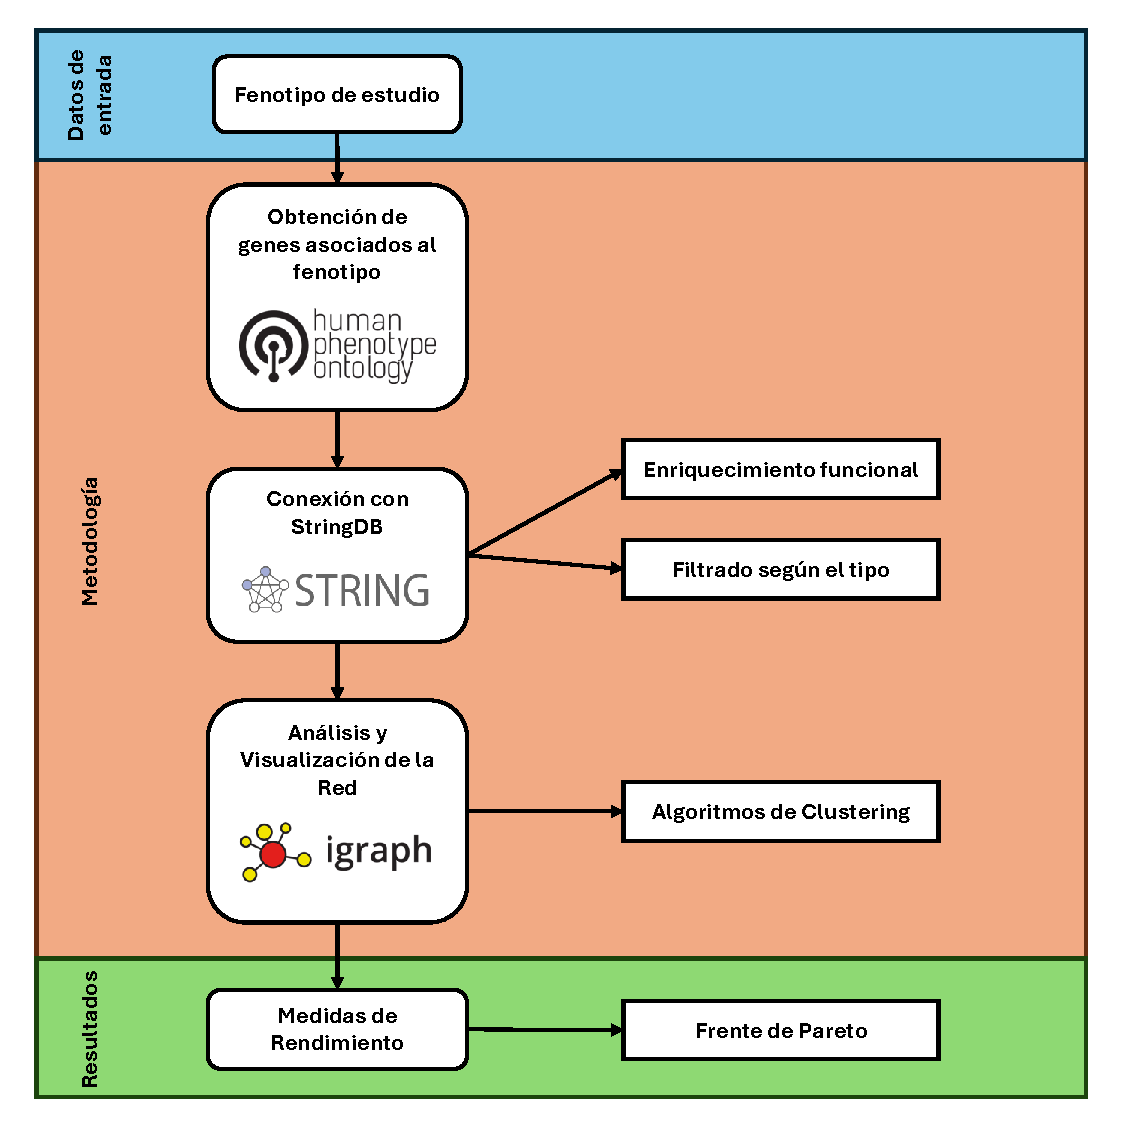
\includegraphics[width=1\linewidth]{figures/methods/Flujo_de_trabajo.pdf}
	\caption{Flujo de trabajo que se seguirá durante el desarrollo del proyecto, partiendo del fenotipo como dato de entrada, metodología y análisis de resultados.}
	\label{fig:flujo_trabajo}
\end{figure}
